% --------------------------------------------------------------
%  reportpreamble.tex – McMaster University report formatting
% --------------------------------------------------------------
% ---- Core document class -----------------------------------------
\documentclass[12pt,oneside]{article}   % 12 pt, single‑sided

% ---- Packages ---------------------------------------------------
\usepackage[utf8]{inputenc}
\usepackage[T1]{fontenc}
\usepackage{lmodern}            % Times‑like font (McMaster default)
\usepackage[english]{babel}
\usepackage{geometry}
\geometry{
  a4paper,
  left=1in,
  right=1in,
  top=1in,
  bottom=1in
}
\usepackage{setspace}
\onehalfspacing                 % 1.5 line spacing (McMaster requirement)

\usepackage{graphicx}
\usepackage{hyperref}
\hypersetup{
  colorlinks=true,
  linkcolor=black,
  citecolor=black,
  urlcolor=black,
  pdfauthor={Yangyang Zhang, Maximilian Fuchs, Seyedmohamad Mirhoseininejad},
  pdftitle={FitCoachAR: Real‑Time Adaptive Exercise Coaching},
  pdfsubject={CAS 772 – Mobile Data Analytics},
  pdfkeywords={pose estimation, AR feedback, exercise coaching}
}

\usepackage{amsmath,amssymb}
\usepackage{url}
\usepackage{natbib}
\bibliographystyle{apalike}      % author‑year style (McMaster preferred)
\usepackage{booktabs}            % for professional tables (\toprule, \midrule, \bottomrule)

\usepackage{tikz}
\usetikzlibrary{shapes.geometric,arrows,positioning}

% ---- Custom style package (your own macros) --------------------
\usepackage{reportformat}       % contains \code{}, \filepath{}, etc.

% ---- Title and author block ------------------------------------
\title{FitCoachAR: Real‑Time Adaptive Exercise Coaching via Pose Estimation and AR Feedback}
\author{
  Yangyang Zhang\thanks{Department of Computer Science, McMaster University} \and
  Maximilian Fuchs\thanks{Department of Computer Science, McMaster University} \and
  Seyedmohamad Mirhoseininejad\thanks{Department of Computer Science, McMaster University}
}
\date{CAS 772 – Mobile Data Analytics \\ \today}
% --------------------------------------------------------------
   % <-- McMaster formatting configuration

\begin{document}
\maketitle

\begin{abstract}
We present \textbf{FitCoachAR}, a real-time adaptive exercise coaching system that combines lightweight pose estimation with augmented-reality feedback and LLM-powered coaching.
The system addresses key limitations of existing fitness applications: lack of real-time corrective feedback, sensitivity to viewpoint changes, and shallow semantic analysis.
Our contributions are threefold.
First, we benchmark multiple pose estimation backends and propose a four-step post-processing pipeline (body-centric canonicalization, yaw compensation, adaptive temporal smoothing, and anatomical consistency projection) that substantially improves joint-angle accuracy and cross-view stability without increasing inference latency.
Second, we introduce \textbf{FormScript}, a semantic intermediate representation that transforms raw pose measurements into interpretable \emph{FormCodes}, which are discrete biomechanical descriptors enabling rule-based form analysis and exercise-specific reasoning.
A short calibration phase personalizes range-of-motion thresholds to each user.
These FormCodes drive both real-time AR-based corrective feedback and \textbf{LLM-powered post-workout summaries} (Llama 3.3 70B via Cerebras), which synthesize per-rep feedback into personalized coaching recommendations.
Third, we validate the FormCode system on the RepCount dataset (101 squat videos, 969 repetitions), achieving biomechanically plausible classifications through data-driven threshold optimization.
Together, these components enable stable, interpretable, and interactive exercise coaching on consumer-grade hardware.
\end{abstract}

% ---- Front‑matter ------------------------------------------------
\pagenumbering{roman}
\clearpage
\tableofcontents
\clearpage
\pagenumbering{arabic}

% ---- Main sections ------------------------------------------------
\clearpage
\section{Introduction}

Home and gym fitness applications increasingly employ AI-based pose estimation to count exercise repetitions, yet most still lack real-time, adaptive coaching on movement quality.
Early research systems such as Pose Trainer~\cite{chen2020pose} and AIFit~\cite{fieraru2021aifit} demonstrate that 3D pose analysis can detect posture errors and evaluate performance, but their pipelines remain largely offline, relying on recorded videos and computationally heavy 3D reconstruction.
As a result, these systems provide limited personalization and cannot adapt feedback dynamically during a workout.
More recent work such as ARFit~\cite{mandic2023arfit} integrates augmented-reality visualization to guide users through motion sequences, but still applies generic thresholds and lacks quantitative evaluation of performance consistency across repetitions and viewpoints.

Commercial applications (e.g., Top Pushup~\cite{toppushup}, QuickPose~\cite{quickpose}) have popularized real-time motion counting and form tracking using smartphone cameras.
However, their analysis is typically shallow, focusing on repetition detection or coarse form classification without distinguishing good versus poor repetitions, assessing tempo stability, or tracking joint-level consistency over time.
Moreover, most commercial apps rely on fixed, population-level thresholds and offer limited adaptive or personalized feedback beyond simple prompts.


\textbf{FitCoachAR} aims to bridge the gap between academic models and consumer applications by providing a \textbf{lightweight, real-time, and adaptive coaching system}.
It monitors exercises via 2D pose estimation, detects common form errors, and delivers feedback through \textbf{augmented-reality overlays} and \textbf{coach-style natural language cues}.
The system personalizes its critique level through a short calibration phase and produces both live corrections and post-session summaries.

This project addresses three major motivations:
\begin{itemize}
    \item \textbf{Accessibility}: Eliminate the dependency on motion-capture equipment, camera calibration, and high-end GPUs.
    \item \textbf{Personalization}: Adapt thresholds and critique sensitivity ($\delta$) to each user rather than relying on fixed global rules.
    \item \textbf{Interactivity}: Transform static, after-exercise evaluation into \textbf{continuous, real-time feedback} that enhances engagement and training quality.
\end{itemize}

\subsection{System Overview}
Figure~\ref{fig:system_overview} presents the system architecture. The user interacts through the interface, which captures video and displays feedback. The backend performs pose estimation, filtering, and rep counting, then passes data to the feedback engine which returns results to the interface.

\begin{figure}[ht]
\centering
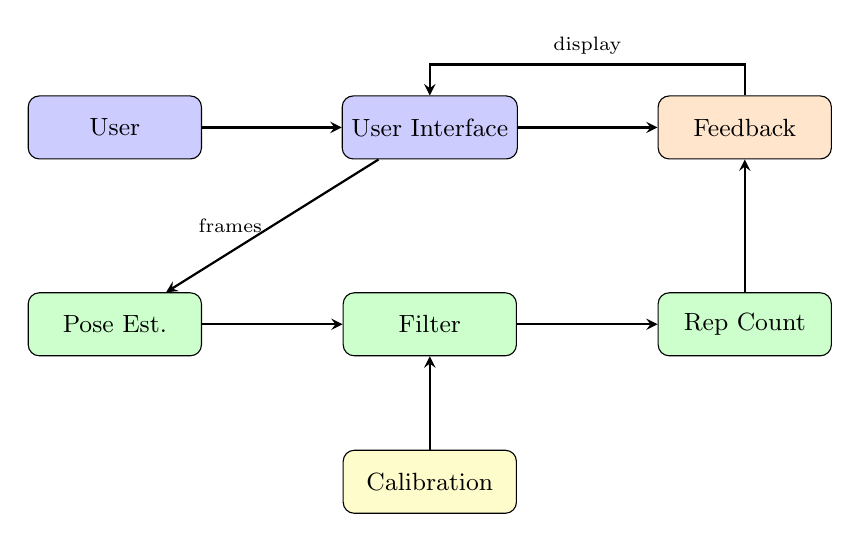
\begin{tikzpicture}[
    box/.style={rectangle, draw, rounded corners, minimum width=2.2cm, minimum height=0.8cm, align=center, font=\small},
    arrow/.style={->, >=stealth, thick}
]

% Top row: User flow
\node[box, fill=blue!20] (user) at (0,0) {User};
\node[box, fill=blue!20] (ui) at (4,0) {User Interface};
\node[box, fill=orange!20] (feedback) at (8,0) {Feedback};

% Bottom row: Processing pipeline
\node[box, fill=green!20] (pose) at (0,-2.5) {Pose Est.};
\node[box, fill=green!20] (filter) at (4,-2.5) {Filter};
\node[box, fill=green!20] (rep) at (8,-2.5) {Rep Count};

% Calibration below
\node[box, fill=yellow!20] (calib) at (4,-4.5) {Calibration};

% Arrows - top row
\draw[arrow] (user) -- (ui);
\draw[arrow] (ui) -- (feedback);
\draw[arrow] (feedback) -- ++(0,0.8) -| node[pos=0.25,above,font=\scriptsize]{display} (ui);

% Arrows - UI to processing
\draw[arrow] (ui) -- node[left,font=\scriptsize]{frames} (pose);

% Arrows - processing pipeline
\draw[arrow] (pose) -- (filter);
\draw[arrow] (filter) -- (rep);
\draw[arrow] (rep) -- (feedback);

% Calibration arrow
\draw[arrow] (calib) -- (filter);

\end{tikzpicture}
\caption{FitCoachAR system architecture.}
\label{fig:system_overview}
\end{figure}















\section{Related Work}
\subsection{Academic Systems}
Pose Trainer (2020) \cite{chen2020pose} applied rule-based analysis of 2D skeletons from OpenPose \cite{cao2017realtime} to classify push-ups and squats. While effective for offline evaluation, it operates on recorded videos and uses fixed thresholds, providing no real-time correction or personalization.

AIFit (CVPR 2021) \cite{fieraru2021aifit} introduced the Fit3D motion-capture dataset and a 3D feedback model capable of joint-level error localization using a deviation parameter ($\eta$) to control strictness. However, it depends on full-sequence 3D reconstruction (MubyNet) and produces template-based text feedback, making it computationally expensive and less adaptive.

ARFit (IMWUT 2023) \cite{mandic2023arfit} added mobile AR overlays for pose visualization, showing that spatial feedback improves exercise learning. Yet, its thresholds remain generic and it lacks quantitative analytics such as repetition consistency or tempo tracking, focusing mainly on visual guidance.

\subsection{Commercial Applications}
Apps like Top Pushup \cite{toppushup} and QuickPose \cite{quickpose} popularized real-time repetition counting using smartphone cameras. Their analysis remains binary—labeling repetitions as correct or incorrect—without distinguishing motion quality, tempo stability, or per-joint improvements. They also rely on static thresholds and simple chatbot-style feedback rather than adaptive, natural-language coaching.

\subsection{Gap Summary}
Across both research and consumer systems, key limitations persist:
\begin{itemize}
    \item Offline or delayed feedback (Pose Trainer, AIFit).
    \item Lack of personalization (global thresholds or $\delta$ not user-specific).
    \item Shallow analysis (no holistic quality metrics).
    \item Limited interactivity (no context-aware language feedback).
\end{itemize}

FitCoachAR addresses these gaps through:
\begin{itemize}
    \item Real-time 2D tracking and online calibration.
    \item Adaptive deviation sensitivity ($\eta$) for user-specific tolerance.
    \item AR-based spatial feedback.
    \item LLM-driven natural coaching for motivating, context-aware guidance.
\end{itemize}
This integration combines AIFit's interpretability with ARFit's usability, achieving real-time, personalized exercise feedback on consumer hardware.

\section{Methodology}

\subsection{Pose Acquisition}
We employ MediaPipe Pose \cite{lugaresi2019mediapipe} for real-time keypoint extraction (33 2D joints). The stream is smoothed using a One-Euro filter to reduce jitter and ensure sub-100 ms latency.

\subsection{Online Repetition Segmentation}
Following AIFit's unsupervised approach, motion periodicity is analyzed from key joint angles (elbow, knee, hip). A simplified online state machine detects phase transitions—descent, bottom, ascent—using derivative sign changes with hysteresis. Each full cycle is labeled as one repetition.

\subsection{Feature Computation and Calibration}
From each repetition we compute angular features:
\begin{itemize}
    \item Active joints: elbows, knees, shoulders (max, min, correlation).
    \item Passive joints: spine and pelvis (mean, standard deviation).
\end{itemize}

During calibration, each key joint or motion phase $i$ is analyzed over three ``best-form'' repetitions:
The mean joint angle is
\begin{equation}
    \bar{U}_i = \frac{1}{3} \sum_{r=1}^{3} \theta_i^{(r)}
\end{equation}

Its deviation percentage from a canonical target $S_i$ is
\begin{equation}
    \eta_i = \frac{\bar{U}_i - S_i}{S_i}
\end{equation}

The pair $(\bar{U}_i, \eta_i)$ forms the personalized baseline and offset for that user.
During runtime, for each joint or phase, the system:
\begin{enumerate}
    \item Measures the current angle $\theta_i$
    \item Computes percentage deviation $e_i = \frac{|\theta_i - \bar{U}_i|}{|\bar{U}_i|}$
\end{enumerate}

A manually set critic parameter $\delta$ determines grading bands:
\begin{itemize}
    \item Good: $e_i < \delta$
    \item Relatively good: $\delta \le e_i < 1.2 \delta$
    \item Bad: $e_i \ge 1.2 \delta$
\end{itemize}

Repetition-level and session-level scores aggregate these joint/phase grades to summarize overall performance.

\subsection{FormScript: Interpretable Feedback via FormCodes}
\label{sec:formscript}

To provide meaningful, explanatory feedback, we implemented ``FormScript'', a rule-based system inspired by the ``PoseScript'' methodology \cite{delmas2022posescript}. The core problem is that simple rep counters don't tell users \textit{how} to improve---users need to know \textit{why} a rep was good or bad. FormScript solves this by discretizing continuous kinematic measurements into human-readable categories (FormCodes) and then applying logical production rules (Super FormCodes) to generate actionable feedback.

\subsubsection{Elementary FormCodes}

Following PoseScript's taxonomy, we define five types of elementary FormCodes. Each FormCode transforms a continuous measurement $v$ into a discrete category based on thresholds. Figure~\ref{fig:formscript-pipeline} illustrates the overall pipeline.

% Block diagram: FormScript Pipeline
\begin{figure}[ht]
\centering
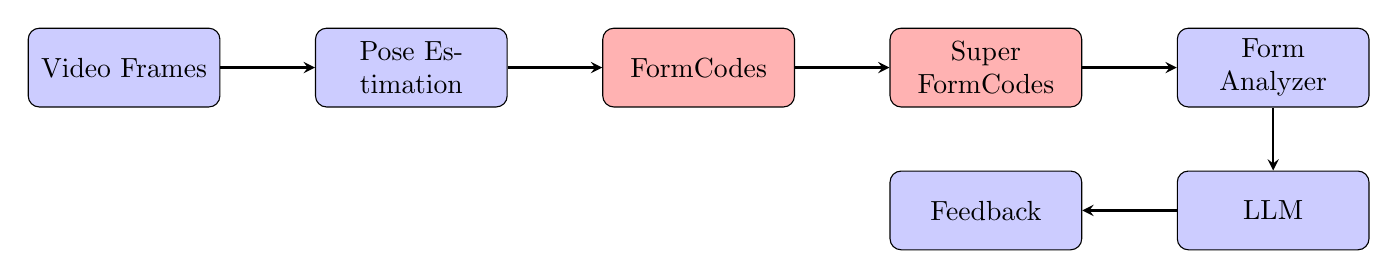
\begin{tikzpicture}[
    node distance=1.2cm,
    block/.style={rectangle, draw, fill=blue!20, text width=2.2cm, text centered, rounded corners, minimum height=1cm},
    arrow/.style={thick,->,>=stealth}
]
% Nodes
\node[block] (video) {Video Frames};
\node[block, right=of video] (pose) {Pose Estimation};
\node[block, right=of pose, fill=red!30] (formcodes) {FormCodes};
\node[block, right=of formcodes, fill=red!30] (super) {Super FormCodes};
\node[block, right=of super] (analyzer) {Form Analyzer};
\node[block, below=0.8cm of analyzer] (llm) {LLM};
\node[block, left=of llm] (feedback) {Feedback};

% Arrows
\draw[arrow] (video) -- (pose);
\draw[arrow] (pose) -- (formcodes);
\draw[arrow] (formcodes) -- (super);
\draw[arrow] (super) -- (analyzer);
\draw[arrow] (analyzer) -- (llm);
\draw[arrow] (llm) -- (feedback);
\end{tikzpicture}
\caption{FormScript pipeline: video frames are processed through pose estimation, discretized into FormCodes, aggregated into Super FormCodes, analyzed, and converted to natural language feedback via LLM.}
\label{fig:formscript-pipeline}
\end{figure}

We categorize FormCodes into two groups based on their nature:

\begin{itemize}
    \item \textbf{Static FormCodes}: Evaluate body geometry (angles, distances, relative positions) on individual frames. While usually assessed at key moments for scoring (e.g., bottom of a squat), they can also be monitored continuously to detect persistent errors.
    \item \textbf{Dynamic FormCodes}: Evaluate motion quality over time (velocity, acceleration, stability) across a sequence of frames.
\end{itemize}

% Block diagram: FormCodes Hierarchy
\begin{figure}[ht]
\centering
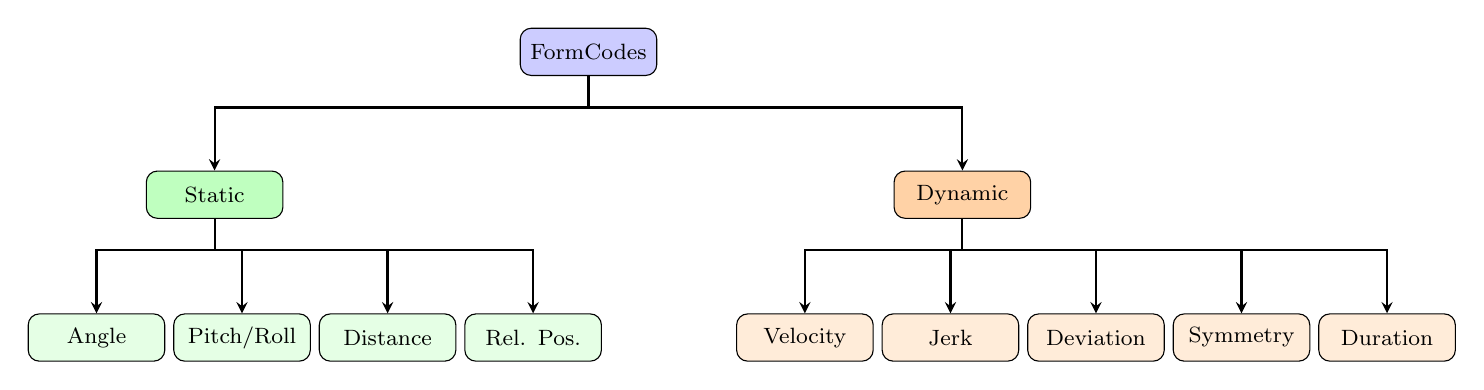
\begin{tikzpicture}[
    node distance=1cm and 0.2cm,
    block/.style={rectangle, draw, text width=1.5cm, text centered, rounded corners, minimum height=0.6cm, font=\footnotesize},
    arrow/.style={thick,->,>=stealth}
]
% Top level
\node[block, fill=blue!20] (formcodes) {FormCodes};

% Second level
\node[block, fill=green!25, below left=1.2cm and 3cm of formcodes] (static) {Static};
\node[block, fill=orange!35, below right=1.2cm and 3cm of formcodes] (dynamic) {Dynamic};

% Static children (4 types)
\node[block, below=1.2cm of static, xshift=-1.5cm, fill=green!10] (angle) {Angle};
\node[block, right=0.1cm of angle, fill=green!10] (pitchroll) {Pitch/Roll};
\node[block, right=0.1cm of pitchroll, fill=green!10] (distance) {Distance};
\node[block, right=0.1cm of distance, fill=green!10] (relpos) {Rel. Pos.};

% Dynamic children (5 types)
\node[block, below=1.2cm of dynamic, xshift=-2cm, fill=orange!15] (velocity) {Velocity};
\node[block, right=0.1cm of velocity, fill=orange!15] (jerk) {Jerk};
\node[block, right=0.1cm of jerk, fill=orange!15] (deviation) {Deviation};
\node[block, right=0.1cm of deviation, fill=orange!15] (symmetry) {Symmetry};
\node[block, right=0.1cm of symmetry, fill=orange!15] (duration) {Duration};

% Arrows - top to second level
\draw[arrow] (formcodes.south) -- ++(0,-0.4) -| (static.north);
\draw[arrow] (formcodes.south) -- ++(0,-0.4) -| (dynamic.north);

% Arrows - Static to children
\draw[arrow] (static.south) -- ++(0,-0.4) -| (angle.north);
\draw[arrow] (static.south) -- ++(0,-0.4) -| (pitchroll.north);
\draw[arrow] (static.south) -- ++(0,-0.4) -| (distance.north);
\draw[arrow] (static.south) -- ++(0,-0.4) -| (relpos.north);

% Arrows - Dynamic to children
\draw[arrow] (dynamic.south) -- ++(0,-0.4) -| (velocity.north);
\draw[arrow] (dynamic.south) -- ++(0,-0.4) -| (jerk.north);
\draw[arrow] (dynamic.south) -- ++(0,-0.4) -| (deviation.north);
\draw[arrow] (dynamic.south) -- ++(0,-0.4) -| (symmetry.north);
\draw[arrow] (dynamic.south) -- ++(0,-0.4) -| (duration.north);
\end{tikzpicture}
\caption{FormCode hierarchy: Static (4 types) for spatial geometry; Dynamic (5 types) for temporal motion quality.}
\label{fig:formcode-taxonomy}
\end{figure}

\paragraph{Static FormCodes}

Static FormCodes analyze body geometry based on individual frames. While some are checked continuously (e.g., torso lean), others are critical at specific key moments (e.g., squat depth). They are adapted from PoseScript's posecode categories.

\subparagraph{Angle FormCodes}
Measure joint flexion at key moments during exercise.

\begin{table}[h]
\centering
\small
\begin{tabular}{|l|l|l|}
\hline
\textbf{Categorization} & \textbf{Condition} & \textbf{Applied To} \\
\hline
completely bent & $v \pm 5 \leq 45$ & L/R-knee, L/R-elbow \\
almost completely bent & $45 < v \pm 5 \leq 75$ & L/R-knee, L/R-elbow \\
bent at right angle & $75 < v \pm 5 \leq 105$ & L/R-knee, L/R-elbow \\
partially bent & $105 < v \pm 5 \leq 135$ & L/R-knee, L/R-elbow \\
slightly bent & $135 < v \pm 5 \leq 160$ & L/R-knee, L/R-elbow \\
straight & $v \pm 5 > 160$ & L/R-knee, L/R-elbow \\
\hline
\end{tabular}
\caption{Angle FormCode categorizations with noise tolerance $\pm 5^\circ$.}
\label{tab:angle-formcodes}
\end{table}

\paragraph{Distance FormCodes}
Measure relative spacing between body parts.

\begin{table}[h]
\centering
\small
\begin{tabular}{|l|l|l|}
\hline
\textbf{Categorization} & \textbf{Condition (m)} & \textbf{Applied To} \\
\hline
close & $v \pm 0.05 \leq 0.20$ & L/R-elbow vs. torso \\
shoulder width & $0.20 < v \pm 0.05 \leq 0.40$ & L/R-foot, L/R-hand \\
spread & $0.40 < v \pm 0.05 \leq 0.80$ & L/R-knee, L/R-foot \\
wide & $v \pm 0.05 > 0.80$ & L/R-foot stance \\
\hline
\end{tabular}
\caption{Distance FormCode categorizations.}
\label{tab:distance-formcodes}
\end{table}

\paragraph{Relative Position FormCodes}
Measure spatial relationships between joints along X, Y, and Z axes.

\begin{table}[h]
\centering
\small
\begin{tabular}{|l|l|l|}
\hline
\textbf{Axis} & \textbf{Categorization} & \textbf{Condition} \\
\hline
X (lateral) & at the right of / x-ignored / at the left of & $v \pm 0.05 \lessgtr \pm 0.15$ \\
Y (vertical) & below / y-ignored / above & $v \pm 0.05 \lessgtr \pm 0.15$ \\
Z (depth) & behind / z-ignored / in front of & $v \pm 0.05 \lessgtr \pm 0.15$ \\
\hline
\end{tabular}
\caption{Relative position FormCode categorizations along each axis.}
\label{tab:relpos-formcodes}
\end{table}

\paragraph{Pitch \& Roll FormCodes}
Measure body segment orientation relative to vertical.

\begin{table}[h]
\centering
\small
\begin{tabular}{|l|l|l|}
\hline
\textbf{Categorization} & \textbf{Condition} & \textbf{Applied To} \\
\hline
vertical (upright) & $v \pm 5 \leq 10$ & torso, pelvis \\
ignored (leaning) & $10 < v \pm 5 \leq 80$ & torso, pelvis \\
horizontal (bent over) & $v \pm 5 > 80$ & torso, pelvis \\
\hline
\end{tabular}
\caption{Pitch \& roll FormCode categorizations.}
\label{tab:pitchroll-formcodes}
\end{table}

\paragraph{Ground-Contact FormCodes}
Detect whether body parts are in contact with the ground.

\begin{table}[h]
\centering
\small
\begin{tabular}{|l|l|l|}
\hline
\textbf{Categorization} & \textbf{Condition (m)} & \textbf{Applied To} \\
\hline
on the ground & $v \pm 0.05 \leq 0.10$ & L/R-knee, L/R-foot \\
ground-ignored & $v \pm 0.05 > 0.10$ & L/R-knee, L/R-foot \\
\hline
\end{tabular}
\caption{Ground-contact FormCode categorizations.}
\label{tab:ground-formcodes}
\end{table}

\paragraph{Dynamic FormCodes}

Dynamic FormCodes extend PoseScript's static approach to analyze motion quality over time, which is critical for exercise evaluation. We define five Dynamic FormCode types.

\subparagraph{Velocity FormCodes}
Measure the speed of movement phases (descent, ascent, lift, lower).

\begin{table}[h]
\centering
\small
\begin{tabular}{|l|l|l|}
\hline
\textbf{Categorization} & \textbf{Condition} & \textbf{Applied To} \\
\hline
controlled & $v \leq 0.5$ m/s & descent\_speed, ascent\_speed \\
fast & $0.5 < v \leq 1.0$ m/s & descent\_speed, ascent\_speed \\
dive/explosive & $v > 1.0$ m/s & descent\_speed, ascent\_speed \\
\hline
\end{tabular}
\caption{Velocity FormCode categorizations.}
\label{tab:velocity-formcodes}
\end{table}

\subparagraph{Jerk FormCodes}
Measure smoothness via rate of acceleration change.

\begin{table}[h]
\centering
\small
\begin{tabular}{|l|l|l|}
\hline
\textbf{Categorization} & \textbf{Condition} & \textbf{Applied To} \\
\hline
smooth & jerk $\leq 2.5$ m/s$^3$ & movement\_smoothness \\
shaky & $2.5 <$ jerk $\leq 5.0$ m/s$^3$ & movement\_smoothness \\
unstable & jerk $> 5.0$ m/s$^3$ & movement\_smoothness \\
\hline
\end{tabular}
\caption{Jerk FormCode categorizations.}
\label{tab:jerk-formcodes}
\end{table}

\subparagraph{Deviation FormCodes}
Measure maximum deviation from expected path or position.

\begin{table}[h]
\centering
\small
\begin{tabular}{|l|l|l|}
\hline
\textbf{Categorization} & \textbf{Condition} & \textbf{Applied To} \\
\hline
stable & $v \leq 0.05$ m & knee\_stability, path\_arc \\
slight\_wobble & $0.05 < v \leq 0.1$ m & knee\_stability, path\_arc \\
unstable & $v > 0.1$ m & knee\_stability, path\_arc \\
\hline
\end{tabular}
\caption{Deviation FormCode categorizations.}
\label{tab:deviation-formcodes}
\end{table}

\subparagraph{Symmetry FormCodes}
Measure left-right asymmetry during movement.

\begin{table}[h]
\centering
\small
\begin{tabular}{|l|l|l|}
\hline
\textbf{Categorization} & \textbf{Condition} & \textbf{Applied To} \\
\hline
level & $v \leq 0.03$ m & hip\_shift \\
slight\_shift & $0.03 < v \leq 0.07$ m & hip\_shift \\
major\_shift & $v > 0.07$ m & hip\_shift \\
\hline
\end{tabular}
\caption{Symmetry FormCode categorizations.}
\label{tab:symmetry-formcodes}
\end{table}

\subparagraph{Duration FormCodes}
Measure time spent in specific positions.

\begin{table}[h]
\centering
\small
\begin{tabular}{|l|l|l|}
\hline
\textbf{Categorization} & \textbf{Condition} & \textbf{Applied To} \\
\hline
squeeze & $t \geq 0.5$ s & pause\_at\_top \\
touch\_and\_go & $t < 0.5$ s & pause\_at\_top \\
\hline
\end{tabular}
\caption{Duration FormCode categorizations.}
\label{tab:duration-formcodes}
\end{table}

\subsubsection{Super FormCodes: Production Rules}

Super FormCodes aggregate multiple elementary FormCodes using logical production rules. Each Super FormCode defines a high-level body configuration by combining conditions with AND/OR operators.

\begin{table}[h]
\centering
\small
\begin{tabular}{|l|l|p{6cm}|}
\hline
\textbf{Subject} & \textbf{Configuration} & \textbf{Production Rule} \\
\hline
torso & upright & pitch \& roll (pelvis, L-shoulder) = vertical AND pitch \& roll (pelvis, R-shoulder) = vertical \\
\hline
body & bent forward & relativePos Y (L-ankle, neck) = below AND relativePos Z (neck, pelvis) = front \\
\hline
knees & deep squat & angle (L-knee) = completely bent AND angle (R-knee) = completely bent \\
\hline
knees & parallel squat & angle (L-knee) = bent at right angle AND angle (R-knee) = bent at right angle \\
\hline
knees & stable & distance (L-knee, L-foot) = close AND distance (R-knee, R-foot) = close \\
\hline
knees & collapsed & relativePos X (L-knee, L-foot) = at right of OR relativePos X (R-knee, R-foot) = at left of \\
\hline
elbows & anchored & distance (L-elbow, torso) = close AND distance (R-elbow, torso) = close \\
\hline
elbows & drifting & distance (L-elbow, torso) = spread OR distance (R-elbow, torso) = spread \\
\hline
feet & shoulder width & distance (L-foot, R-foot) = shoulder width AND pitch \& roll (L-foot, R-foot) = horizontal \\
\hline
\end{tabular}
\caption{Super FormCode production rules for exercise analysis.}
\label{tab:super-formcodes}
\end{table}

\subsubsection{Exercise-Specific FormCode Application}

\paragraph{Squat Analysis}
Key FormCodes monitored: knee angle (depth), torso pitch (lean), knee-to-foot distance (stability), hip levelness (asymmetry).

\paragraph{Bicep Curl Analysis}
Key FormCodes monitored: elbow angle (contraction), elbow-to-torso distance (anchoring), shoulder/hip pitch (swing detection), wrist angle (neutral grip).

\subsubsection{Configuration-Driven Definition}

A key strength of the FormScript framework is its extensibility. Rather than hard-coding rules, all FormCodes and Super FormCodes are defined in external configuration files, making it easy for domain experts (e.g., physiotherapists) to adjust thresholds or add new exercises without modifying the core codebase.

\paragraph{Elementary Configuration}
The \texttt{form\_codes\_config.py} file defines the primitives for each exercise. Each entry specifies the measurement type, units, and strict categorization thresholds. For example, the configuration for squat depth is defined as:

\begin{verbatim}
"squat_depth": {
    "type": "angle",
    "description": "Angle of the knee joint...",
    "categories": [
        {"name": "deep", "v_max": 90},
        {"name": "parallel", "v_min": 90, "v_max": 110},
        {"name": "shallow", "v_min": 110}
    ]
}
\end{verbatim}

\paragraph{Production Rule Configuration}
The \texttt{super\_form\_codes\_config.py} file defines high-level states using logical rules. These rules specify which elementary FormCode categories must be present (\texttt{must\_be}) or absent (\texttt{must\_not\_be}).

\begin{verbatim}
"GOOD_REP": {
    "description": "A well-executed squat...",
    "rules": [
        {"form_code": "squat_depth", "must_be": ["deep"]},
        {"form_code": "knee_stability", 
         "must_not_be": ["unstable", "slight_wobble"]},
        {"form_code": "torso_angle", 
         "must_not_be": ["bent_over", "leaning"]}
    ]
}
\end{verbatim}

This data-driven approach decouples the biomechanical definitions from the pose estimation logic, similar to the PoseScript architecture \cite{delmas2022posescript}.

\subsubsection{Feedback Systems}

The FormScript pipeline feeds into two complementary feedback paths: real-time coaching during exercise and offline analysis after workout completion.

\paragraph{Real-Time Feedback}
During exercise, feedback must maintain sub-100ms latency. The system provides:

\begin{enumerate}
    \item \textbf{Post-Rep Commands}: After each repetition, Super FormCodes are mapped to concise coaching commands. For example:
    \begin{itemize}
        \item BODY\_SWING $\rightarrow$ ``No swinging! Use your bicep only.''
        \item ELBOW\_DRIFT $\rightarrow$ ``Pin your elbow to your side!''
        \item SHALLOW\_SQUAT $\rightarrow$ ``Go deeper!''
        \item KNEE\_CAVE $\rightarrow$ ``Knees out!''
    \end{itemize}
    
    \item \textbf{Guidance Arrows}: Visual AR overlays on the skeleton showing direction of correction:
    \begin{itemize}
        \item Arrow on wrist pointing up for INCOMPLETE\_RANGE
        \item Arrow on knee pointing outward for KNEE\_CAVE
        \item Arrow on hip pointing down for SHALLOW\_SQUAT
    \end{itemize}
    
    \item \textbf{Joint Highlighting}: Problematic joints are highlighted in red on the skeleton overlay.
\end{enumerate}

\paragraph{Offline Feedback (Post-Workout)}
After the workout session, accumulated FormCode data from all repetitions is processed for comprehensive analysis:

\begin{enumerate}
    \item \textbf{Per-Rep Feedback Generation}: Each repetition's FormCodes are converted to human-readable sentences. For example:
    \begin{itemize}
        \item peak\_flexion = full\_contraction $\rightarrow$ ``You achieved a full muscle contraction at the top of the curl.''
        \item swing\_momentum = body\_swing $\rightarrow$ ``Significant body swing detected---you're using momentum instead of muscle.''
    \end{itemize}
    
    \item \textbf{LLM-Powered Session Summary}: All repetition data is aggregated and sent to an LLM (Llama 3.3 70B via Cerebras) to generate a natural language summary:
    \begin{itemize}
        \item Total reps and form score
        \item Most common issues with actionable tips
        \item Encouraging motivation for next session
    \end{itemize}
    
    \item \textbf{Q\&A Capability}: Users can ask follow-up questions about their workout (e.g., ``How was my elbow position?'') and receive personalized responses based on their session data.
\end{enumerate}

This dual-path approach ensures users receive immediate, actionable feedback during exercise while benefiting from comprehensive LLM-generated insights after workout completion.


\section{Qualitative Results}
\label{sec:results}

We conducted a live demonstration of the FitCoachAR system to validate its core components: real-time visual feedback, quantitative form analysis, and generative AI coaching. The following results illustrate the system's output during a standard workout session (Bicep Curls and Squats).

\subsubsection{Real-Time Visual Feedback}
The primary contribution of FitCoachAR is the low-latency Augmented Reality overlay. Figure \ref{fig:ar_arrows} demonstrates the system's ability to detect form errors in real-time. In this example (Bicep Curl), the system detected "Elbow Drift" and immediately rendered a directional arrow guiding the user to tuck their elbow in. This visual cue is generated within 100ms, providing instant correction without interrupting the exercise flow.

\begin{figure}[h]
    \centering
    \includegraphics[width=0.8\textwidth]{figures/arrow.png}
    \caption{Real-time AR feedback mechanism. The system detects an elbow stability error and superimposes a yellow arrow on the user's arm, directing them to correct their form.}
    \label{fig:ar_arrows}
\end{figure}

\subsection{Quantitative Form Analysis}
After completing a set, the system compiles a detailed "Form Analysis" report. Figure \ref{fig:form_analysis} shows the post-set summary screen. The system aggregates data from all repetitions to calculate an overall "Form Score" (e.g., 90\%). It also provides a breakdown of specific issues, such as "Body Swing" or "Incomplete Range," along with a rep-by-rep analysis. This allows users to identify consistent patterns in their technique.

\begin{figure}[h]
    \centering
    \includegraphics[width=0.8\textwidth]{figures/form-analysis.png}
    \caption{Post-workout Form Analysis summary. The interface displays an overall score, a breakdown of detected errors (e.g., Body Swing), and a detailed log of each repetition.}
    \label{fig:form_analysis}
\end{figure}

\subsection{Generative AI Coaching}
To provide deeper insights, FitCoachAR integrates a Large Language Model (LLM) as a virtual coach. Figure \ref{fig:ai_coach} shows the chat interface where the user can ask questions about their performance. The LLM receives the structured workout data (FormCodes) and provides natural language advice. In this instance, the coach offers specific tips on how to fix the "Body Swing" issue detected during the set.

\begin{figure}[h]
    \centering
    \includegraphics[width=0.8\textwidth]{figures/ai-response.png}
    \caption{Generative AI Coach interface. The user interacts with the LLM to receive personalized, actionable advice based on the workout data.}
    \label{fig:ai_coach}
\end{figure}

\subsection{Data Processing pipeline}
Underlying these visual interfaces is a robust data processing pipeline. Figure \ref{fig:script_response} visualizes the raw JSON outputs generated by the FormScript engine. These structured responses confirm that the system correctly translates raw pose landmarks into semantic "Super FormCodes" (e.g., \texttt{GOOD\_REP}, \texttt{ELBOW\_DRIFT}), which then drive both the AR arrows and the AI coaching.

\begin{figure}[h]
    \centering
    \includegraphics[width=0.8\textwidth]{figures/script-responses.png}
    \caption{Backend data processing logs. The JSON output confirms the detection of specific FormCodes, verifying the accuracy of the rule-based evaluation engine.}
    \label{fig:script_response}
\end{figure}

\subsection{FormCode Validation and Threshold Optimization}
To validate the FormCode system's effectiveness and calibration accuracy, we conducted comprehensive testing on the RepCount dataset~\cite{dwibedi2020repcount}, analyzing 101 squat videos comprising 969 repetitions. This validation employed a data-driven threshold optimization methodology to ensure biomechanically plausible classifications.

\subsubsection{Validation Procedure}
Following per-video calibration using the first 2 repetitions to establish personalized range-of-motion (ROM) thresholds, we extracted 4 FormCodes (squat\_depth, knee\_stability, torso\_angle, hip\_shift) for each remaining repetition. The pipeline was modified to save raw metric values alongside categorical classifications, enabling distribution analysis.

Our threshold optimization process involved: (1) extracting raw metric distributions from all 969 squat bottoms, (2) analyzing percentiles to identify biomechanically appropriate boundaries, and (3) validating optimized thresholds through full dataset re-analysis. For example, knee\_stability thresholds were adjusted from 0.9-1.1 to 0.81-1.21 (15th-85th percentile of the knee valgus ratio distribution), increasing stable classification from 33.3\% to 68.9\%. Similarly, torso\_angle thresholds were relaxed from $<$20° to $<$45° for upright posture, increasing classification from 12.2\% to 63.7\% to reflect natural squat biomechanics where some forward lean is both normal and desirable.

\subsubsection{Optimization Results}
Figure \ref{fig:formcode_distribution} presents the final FormCode distributions. All FormCodes achieved \textbf{100\% coverage} across repetitions, with multi-category activation spanning 2-3 categories per FormCode. The optimized distributions demonstrate biomechanically plausible results: 94.5\% deep squats (indicating effective personalized ROM calibration), 68.9\% stable knee tracking, 63.7\% upright torso posture, and 48.7\% level hips. Consistency metrics range from 48.7\% to 94.5\%, appropriately capturing different aspects of movement control—high consistency for depth (reflecting reliable ROM achievement) and moderate consistency for knee stability (reflecting expected inter-rep variability in joint control).

\begin{figure}[h]
\centering
\includegraphics[width=0.95\textwidth]{figures/formcode_analysis_PUBLICATION.png}
\caption{FormCode distribution analysis across 969 squat repetitions from RepCount dataset. All FormCodes demonstrate 100\% coverage with multi-category distributions: (a) squat\_depth shows 94.5\% deep squats via personalized calibration, (b) knee\_stability exhibits 68.9\% stable tracking with data-driven thresholds, (c) torso\_angle shows 63.7\% upright posture, and (d) hip\_shift displays 48.7\% level hips. Consistency percentages annotated in each panel range from 48.7\% to 94.5\%, reflecting varying biomechanical control across metrics.}
\label{fig:formcode_distribution}
\end{figure}

Table \ref{tab:formcode_performance} summarizes the performance metrics. The data-driven optimization methodology successfully balanced sensitivity (multi-category discrimination) with biomechanical realism, validating the production implementation's ability to provide meaningful, individualized form feedback across diverse users.

\begin{table}[h]
\centering
\caption{FormCode Performance Metrics on RepCount Dataset (101 videos, 969 reps)}
\label{tab:formcode_performance}
\begin{tabular}{lcccc}
\toprule
\textbf{FormCode} & \textbf{Coverage} & \textbf{Consistency} & \textbf{Categories} & \textbf{Optimization} \\
\midrule
squat\_depth & 100.0\% & 94.5\% & 3 & Per-video calibration \\
knee\_stability & 100.0\% & 68.9\% & 3 & Data-driven (percentile) \\
torso\_angle & 100.0\% & 63.7\% & 3 & Data-driven (percentile) \\
hip\_shift & 100.0\% & 48.7\% & 3 & Domain expert \\
\bottomrule
\end{tabular}
\end{table}


\section{Discussion and Limitations}
\label{sec:discussion}

\subsection{Biases and Limitations in Model Comparison and Post-Processing Evaluation}

While the proposed post-processing approach demonstrates strong robustness--latency trade-offs
for real-time fitness coaching, several limitations should be acknowledged.
First, our evaluation projects both ground-truth 3D joints and predictions from
3D-based models into a normalized 2D torso-centric plane to enable fair comparison
with 2D pose estimators.
Although this design removes viewpoint bias, it may also suppress the inherent
depth advantages of true 3D models, potentially underestimating their full capability.
Second, discrepancies in joint definitions across datasets and models introduce
additional uncertainty: ground-truth annotations are derived from sensor-based
motion-capture systems, whose joint semantics do not perfectly align with those of
learning-based 2D estimators such as MoveNet, MediaPipe, or ROMP.

Third, the four proposed post-processing techniques were evaluated as a combined
pipeline, without a dedicated ablation study to isolate the individual contribution
of each component.
While this choice reflects our system-oriented focus on end-to-end performance,
it limits fine-grained attribution of improvements.
Finally, the high dimensionality of pose data—spanning multiple joints, frames,
viewpoints, and exercises—was summarized using global metrics.
Such aggregation may obscure phase-specific or viewpoint-specific behaviors,
particularly for exercises where joint dynamics vary substantially across motion phases.

\section{Division of Labor}
\label{sec:division-of-labor}

This project was completed as a group effort. Below we summarize the workload division.

\paragraph{Yangyang Zhang.}
Yangyang's primary responsibilities include:
\begin{itemize}
    \item Establishing the core frontend--backend streaming pipeline (e.g., WebSocket-based frame delivery and latency reduction), along with primary front-end UI design and the initial AR overlay/markers.
    \item Design and proposal of the four lightweight post-processing techniques (reported in Sec.~\ref{sec:model-eval}) for stabilizing MoveNet~2D outputs.
    \item Empirical model analysis and experiments reported in Sec.~\ref{sec:movenet-postproc}, covering multi-backend benchmarking, stability evaluation, and latency measurement.
\end{itemize}

\paragraph{Seyedmohamad Mirhoseininejad.}
Seyedmohamad's primary responsibilities include:
\begin{itemize}
    \item Design and implementation of the FormScript feedback system, including elementary FormCodes and Super FormCodes for rule-based form analysis.
    \item Development of the calibration system for personalized range-of-motion thresholds.
    \item Integration of LLM-powered post-workout summaries using Llama 3.3 70B via Cerebras, including per-rep feedback aggregation.
    \item FormCode validation experiments on the RepCount dataset (Sec.~4.6).
\end{itemize}

\paragraph{Maximilian Fuchs.}
Please fill in the corresponding responsibilities for the remaining members (e.g., backend services, calibration logic, repetition segmentation, LLM feedback, and report writing) to keep the report self-contained.

\section{Conclusion}

This project presented \textbf{FitCoachAR}, a real-time, adaptive exercise coaching system that bridges the gap between academic pose-analysis pipelines and practical consumer fitness applications.

Through a comprehensive empirical evaluation, we showed that among a wide range of pose estimation backends,
\textbf{MoveNet\_2D} offers the most favorable accuracy--latency trade-off for real-time use.
More importantly, our four-step post-processing pipeline—body-centric canonicalization,
yaw compensation, confidence-/motion-adaptive temporal smoothing, and anatomical consistency projection—
substantially improves both joint-angle accuracy and cross-view stability without increasing inference latency.

Beyond low-level pose accuracy, FitCoachAR introduces \textbf{FormScript}, a semantic intermediate representation that transforms continuous pose measurements into interpretable FormCodes.
This abstraction enables exercise-specific reasoning, personalized calibration, and natural-language feedback,
supporting both real-time corrective cues and post-workout summaries.
By decoupling biomechanical definitions from pose estimation and feedback generation,
FormScript provides a flexible and extensible framework for future exercise analysis systems.

Overall, FitCoachAR illustrates a practical design philosophy for interactive human-motion applications:
prioritizing robustness, interpretability, and responsiveness over raw model complexity.
While several limitations remain—including the lack of ablation analysis and the reliance on aggregated metrics—
the results suggest that integrated, lightweight post-processing can significantly narrow the gap
between small 2D models and heavier 3D approaches in real-world fitness coaching scenarios.

Future work may explore finer-grained phase-specific evaluation, user studies on coaching effectiveness,
and the extension of FormCodes to rehabilitation and clinical movement assessment.
Nonetheless, this project demonstrates that real-time, personalized, and explainable exercise coaching
is achievable on consumer hardware using principled pose processing and semantic reasoning.


% ---- Bibliography -------------------------------------------------
\bibliography{references}

% ---- Appendices ---------------------------------------------------
\clearpage
\appendix

% Configure table numbering for appendix (A1, A2, A3, ...)
\renewcommand{\thetable}{A\arabic{table}}
\setcounter{table}{0}

\section{FormCode Reference Tables}
\label{appendix:formcodes}

This appendix provides a complete reference of all FormCode categorizations used in the FormScript system. Each table defines the discrete categories, threshold conditions, and applicable body parts for a specific FormCode type.

\subsection{Static FormCodes}

Static FormCodes evaluate body geometry on individual frames.

\subsubsection{Angle FormCodes}
Measure joint flexion at key moments during exercise.

\begin{table}[h]
\caption{Angle FormCode categorizations with noise tolerance $\pm 5^\circ$.}
\label{tab:angle-formcodes}
\centering
\small
\begin{tabular}{|l|l|l|}
\hline
\textbf{Categorization} & \textbf{Condition} & \textbf{Applied To} \\
\hline
completely bent & $v \pm 5 \leq 45$ & L/R-knee, L/R-elbow \\
almost completely bent & $45 < v \pm 5 \leq 75$ & L/R-knee, L/R-elbow \\
bent at right angle & $75 < v \pm 5 \leq 105$ & L/R-knee, L/R-elbow \\
partially bent & $105 < v \pm 5 \leq 135$ & L/R-knee, L/R-elbow \\
slightly bent & $135 < v \pm 5 \leq 160$ & L/R-knee, L/R-elbow \\
straight & $v \pm 5 > 160$ & L/R-knee, L/R-elbow \\
\hline
\end{tabular}
\end{table}

\subsubsection{Distance FormCodes}
Measure relative spacing between body parts.

\begin{table}[h]
\caption{Distance FormCode categorizations.}
\label{tab:distance-formcodes}
\centering
\small
\begin{tabular}{|l|l|l|l|}
\hline
\textbf{Categorization} & \textbf{Condition} & \textbf{Unit} & \textbf{Applied To} \\
\hline
narrow & $v < 0.9$ & ratio & stance width (feet) \\
shoulder\_width & $0.9 \leq v \leq 1.2$ & ratio & stance width (feet) \\
wide & $v > 1.2$ & ratio & stance width (feet) \\
anchored & $v \leq 0.08$ & normalized & elbow drift \\
slight\_drift & $0.08 < v \leq 0.15$ & normalized & elbow drift \\
major\_drift & $v > 0.15$ & normalized & elbow drift \\
\hline
\end{tabular}
\end{table}

\subsubsection{Relative Position FormCodes}
Measure spatial relationships between joints along X, Y, and Z axes.

\begin{table}[h]
\caption{Relative position FormCode categorizations.}
\label{tab:relpos-formcodes}
\centering
\small
\begin{tabular}{|l|l|l|}
\hline
\textbf{Measurement} & \textbf{Categorization} & \textbf{Condition} \\
\hline
Knee forward travel (Z-axis) & behind\_toes & $v \leq 0$ m \\
Knee forward travel (Z-axis) & over\_toes & $v > 0$ m \\
\hline
\end{tabular}
\end{table}

\subsubsection{Pitch \& Roll FormCodes}
Measure body segment orientation relative to vertical.

\begin{table}[h]
\caption{Pitch \& roll FormCode categorizations.}
\label{tab:pitchroll-formcodes}
\centering
\small
\begin{tabular}{|l|l|l|}
\hline
\textbf{Categorization} & \textbf{Condition} & \textbf{Applied To} \\
\hline
vertical (upright) & $v \pm 5 \leq 10$ & torso, pelvis \\
ignored (leaning) & $10 < v \pm 5 \leq 80$ & torso, pelvis \\
horizontal (bent over) & $v \pm 5 > 80$ & torso, pelvis \\
\hline
\end{tabular}
\end{table}

\subsubsection{Ground-Contact FormCodes}
Detect whether body parts are in contact with the ground.

\begin{table}[h]
\caption{Ground-contact FormCode categorizations.}
\label{tab:ground-formcodes}
\centering
\small
\begin{tabular}{|l|l|l|}
\hline
\textbf{Categorization} & \textbf{Condition (m)} & \textbf{Applied To} \\
\hline
on the ground & $v \pm 0.05 \leq 0.10$ & L/R-knee, L/R-foot \\
ground-ignored & $v \pm 0.05 > 0.10$ & L/R-knee, L/R-foot \\
\hline
\end{tabular}
\end{table}

\subsection{Dynamic FormCodes}

Dynamic FormCodes evaluate motion quality over temporal windows.

\subsubsection{Velocity FormCodes}
Measure the speed of movement phases (descent, ascent, lift, lower).

\begin{table}[h]
\caption{Velocity FormCode categorizations.}
\label{tab:velocity-formcodes}
\centering
\small
\begin{tabular}{|l|l|l|}
\hline
\textbf{Categorization} & \textbf{Condition} & \textbf{Applied To} \\
\hline
controlled & $v \leq 0.5$ m/s & descent\_speed, ascent\_speed \\
fast & $0.5 < v \leq 1.0$ m/s & descent\_speed, ascent\_speed \\
dive/explosive & $v > 1.0$ m/s & descent\_speed, ascent\_speed \\
\hline
\end{tabular}
\end{table}

\subsubsection{Jerk FormCodes}
Measure smoothness via rate of acceleration change.

\begin{table}[h]
\caption{Jerk FormCode categorizations.}
\label{tab:jerk-formcodes}
\centering
\small
\begin{tabular}{|l|l|l|}
\hline
\textbf{Categorization} & \textbf{Condition} & \textbf{Applied To} \\
\hline
smooth & jerk $\leq 2.5$ m/s$^3$ & movement\_smoothness \\
shaky & $2.5 <$ jerk $\leq 5.0$ m/s$^3$ & movement\_smoothness \\
unstable & jerk $> 5.0$ m/s$^3$ & movement\_smoothness \\
\hline
\end{tabular}
\end{table}

\subsubsection{Deviation FormCodes}
Measure maximum deviation from expected path or position.

\begin{table}[h]
\caption{Deviation FormCode categorizations.}
\label{tab:deviation-formcodes}
\centering
\small
\begin{tabular}{|l|l|l|l|}
\hline
\textbf{Categorization} & \textbf{Condition} & \textbf{Unit} & \textbf{Applied To} \\
\hline
stable / clean\_arc & $v \leq 0.05$ & m & knee\_stability, path\_arc \\
slight\_wobble / wandering & $0.05 < v \leq 0.1$ & m & knee\_stability \\
unstable & $v > 0.1$ & m & knee\_stability \\
no\_swing & $v \leq 0.15$ & normalized & swing\_momentum \\
slight\_swing & $0.15 < v \leq 0.25$ & normalized & swing\_momentum \\
body\_swing & $v > 0.25$ & normalized & swing\_momentum \\
\hline
\end{tabular}
\end{table}

\subsubsection{Symmetry FormCodes}
Measure left-right asymmetry during movement.

\begin{table}[h]
\caption{Symmetry FormCode categorizations.}
\label{tab:symmetry-formcodes}
\centering
\small
\begin{tabular}{|l|l|l|}
\hline
\textbf{Categorization} & \textbf{Condition (m)} & \textbf{Applied To} \\
\hline
level & $v \leq 0.03$ & hip\_shift \\
slight\_shift & $0.03 < v \leq 0.07$ & hip\_shift \\
major\_shift & $v > 0.07$ & hip\_shift \\
\hline
\end{tabular}
\end{table}

\subsubsection{Duration FormCodes}
Measure time spent in specific positions.

\begin{table}[h]
\caption{Duration FormCode categorizations.}
\label{tab:duration-formcodes}
\centering
\small
\begin{tabular}{|l|l|l|}
\hline
\textbf{Categorization} & \textbf{Condition} & \textbf{Applied To} \\
\hline
squeeze & $t \geq 0.5$ s & pause\_at\_top \\
touch\_and\_go & $t < 0.5$ s & pause\_at\_top \\
\hline
\end{tabular}
\end{table}


\end{document}
